%%%%%%%%%%%%%%%%%%%%%%%%%%%%
\section{Introduction}
\label{sec:Introduction}
%%%%%%%%%%%%%%%%%%%%%%%%%%%%

\begin{figure}[H]
  \centering
  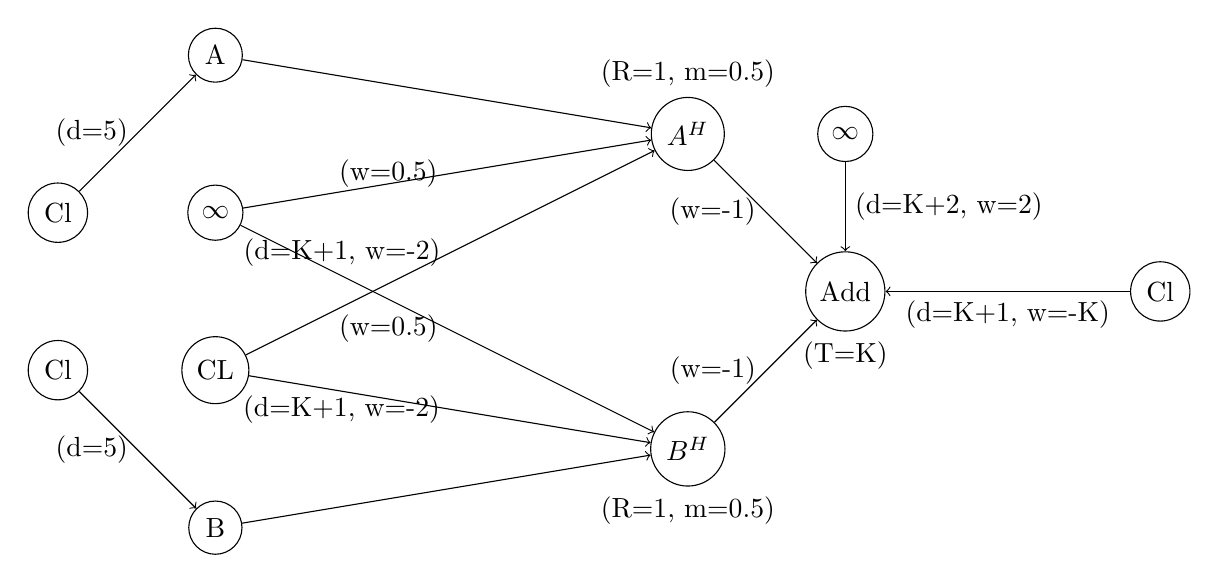
\begin{tikzpicture}
    \node[shape=circle,draw=black] (CL1) at (0,2) {Cl};
    \node[shape=circle,draw=black] (CL2) at (0,4) {Cl};
    
    \node[shape=circle,draw=black] (A) at (2,6) {A};
    \node[shape=circle,draw=black] (Inf1) at (2,4) {$\infty$};
    \node[shape=circle,draw=black] (CL3) at (2,2) {CL};
    \node[shape=circle,draw=black] (B) at (2,0) {B};
  
    \node[shape=circle,draw=black,label=above:{(R=1, m=0.5)}] (AH) at (8,5) {$A^H$};
    \node[shape=circle,draw=black,label=below:{(R=1, m=0.5)}] (BH) at (8,1) {$B^H$};
  
    \node[shape=circle,draw=black] (Inf2) at (10,5) {$\infty$};
    \node[shape=circle,draw=black,label=below:{(T=K)}] (Add) at (10,3) {Add};
  
    \node[shape=circle,draw=black] (CL4) at (14,3) {Cl};
  


    \path [->] (CL2) edge node[left] {(d=5)} (A);
    \path [->] (CL1) edge node[left] {(d=5)} (B);
    \path [->] (A) edge node[left] {} (AH);
    \path [->] (B) edge node[left] {} (BH);
    \path [->] (Inf1) edge node[left] {(w=0.5)} (AH);
    \path [->] (Inf1) edge node[left] {(w=0.5)} (BH);
    \path [->] (CL3) edge node[left] {(d=K+1, w=-2)} (AH);
    \path [->] (CL3) edge node[left] {(d=K+1, w=-2)} (BH);
    \path [->] (AH) edge node[left] {(w=-1)} (Add);
    \path [->] (BH) edge node[left] {(w=-1)} (Add);
    \path [->] (Inf2) edge node[right] {(d=K+2, w=2)} (Add);
    \path [->] (CL4) edge node[below] {(d=K+1, w=-K)} (Add);
  \end{tikzpicture}

\autoref{NotAPinkElephant} shows what a pink elephant does not look like:
\begin{figure}[h]
\begin{center}
	\subfigure[A grey elephant. Definitely not pink.]{\label{GreyElephant} \includegraphics[width=0.33\textwidth]{GreyElephant} }
	\subfigure[A common misconception is that pinkuins are pink. This is not true, as they are not elephants.]{\label{Pinkuin} \includegraphics[width=0.33\textwidth]{Pinkuin} }
	\caption{Non-pink non-elephants.}
	\label{NotAPinkElephant}
\end{center}
\end{figure} 
